% !TEX root = ./technical_doc.tex
\chapter{USE CASE}
The model that will be used based on the requirements is shown in \lccref{fig:rich_picture}. The systems one would like to model using this library may or may not have governing equations that are defined to describe its behavior. In both cases, the measurements of said systems are typically discrete values representing some state of the systems such as temperature distribution. Other measurements may include the thermal conductivity distribution of systems or heat source distribution. Together these form the effect and causes of said system.
\begin{figure}[H]
    \centering
    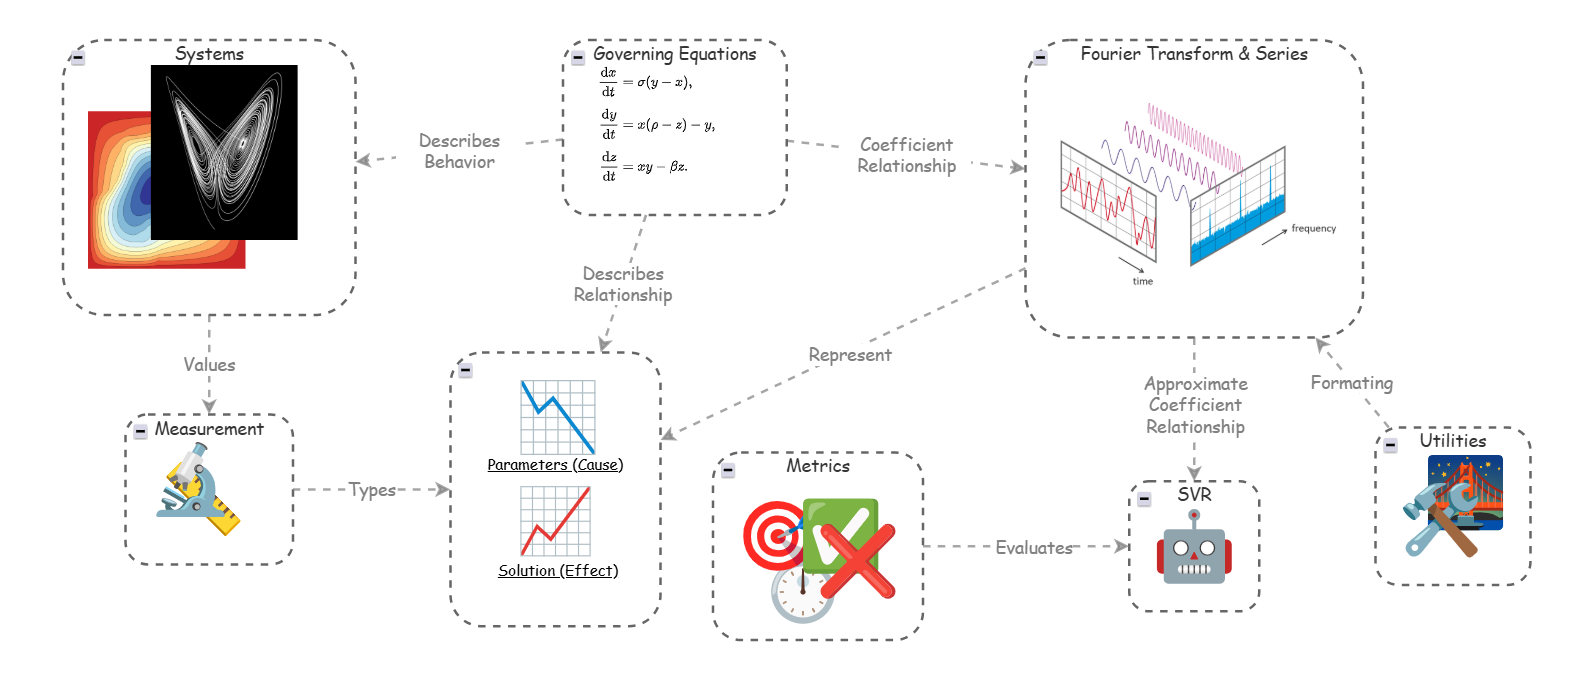
\includegraphics[width=1.0\linewidth]{figures/rich_picture.png}
    \caption{Rich picture diagram illustrating the environment and use case for the library.}\label{fig:rich_picture}
\end{figure}

Functions from measurements or synthetically generated using known governing equations can be represented as the Fourier coefficients of their approximating Fourier series. As the computation must be able to switch between the physical and Fourier domain, other utilities to change the data format will also be essential. Because the relationship between solutions and the parameters can be learned as the relationship between the coefficients of their parameters, the Least-Squares Support Vector Regression is used to learn this from data. Evaluation of how well the model performs will also be required to understand areas of improvement.
